\documentclass[11pt, oneside]{article}
\usepackage{geometry}
\geometry{letterpaper}
\usepackage{graphicx}
\usepackage{amssymb}
\usepackage{amsmath}
\usepackage{tikz}
\usepackage{tikz-qtree}
\usepackage{url}
\usepackage[T1]{fontenc}

\title{SICP Exercise 3.20}
\author{Yuchong Pan}

\begin{document}
\maketitle

The environment structure created by evaluating \textbf{(define x (cons 1 2))} and \textbf{(define z (cons x x))} is given as follows.

\begin{figure}[h!]
    \centering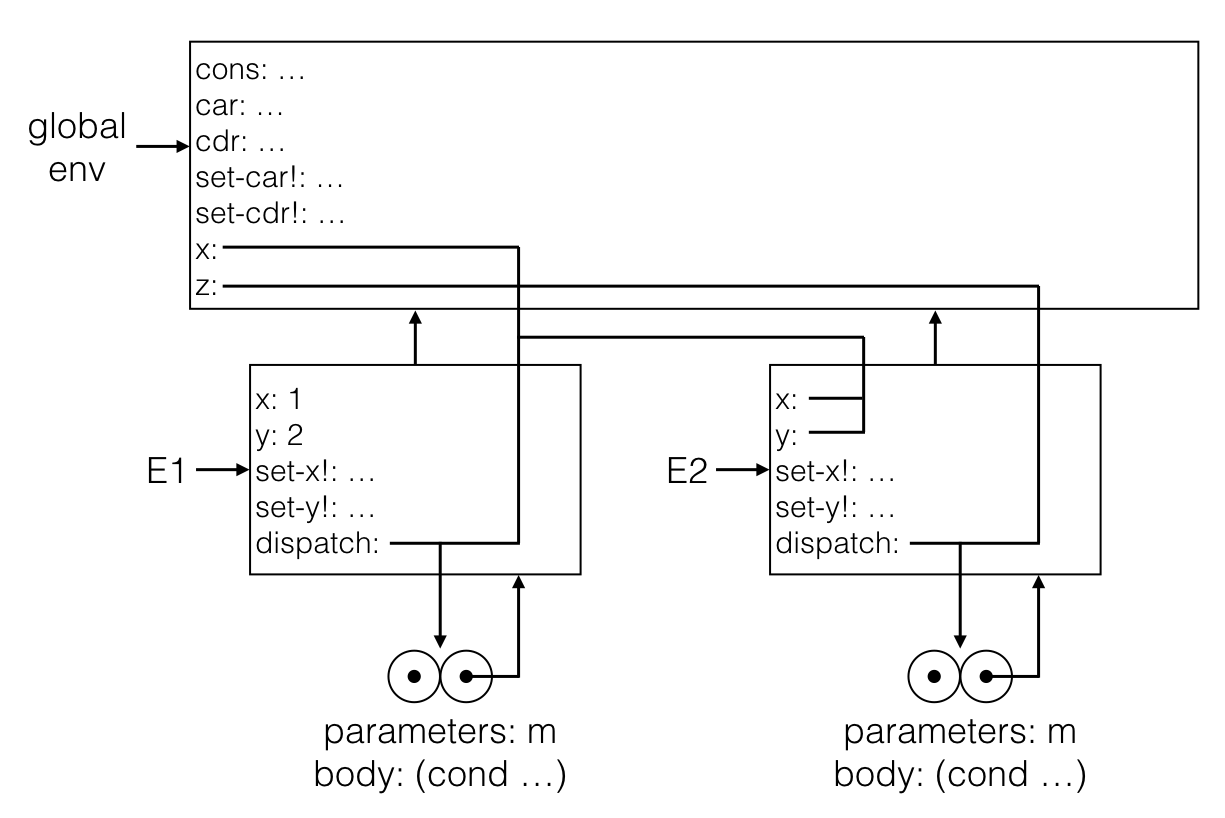
\includegraphics[width=15cm]{ex-3.20-1.png}
    \caption{Effect of \textbf{(define x (cons 1 2))} and \textbf{(define z (cons x x))}.}
\end{figure}

The environment structures created by evaluating \textbf{(set-car! (cdr z) 17)} and by evaluting \textbf{(car x)} are given as follows, respectively.

\begin{figure}[h!]
    \centering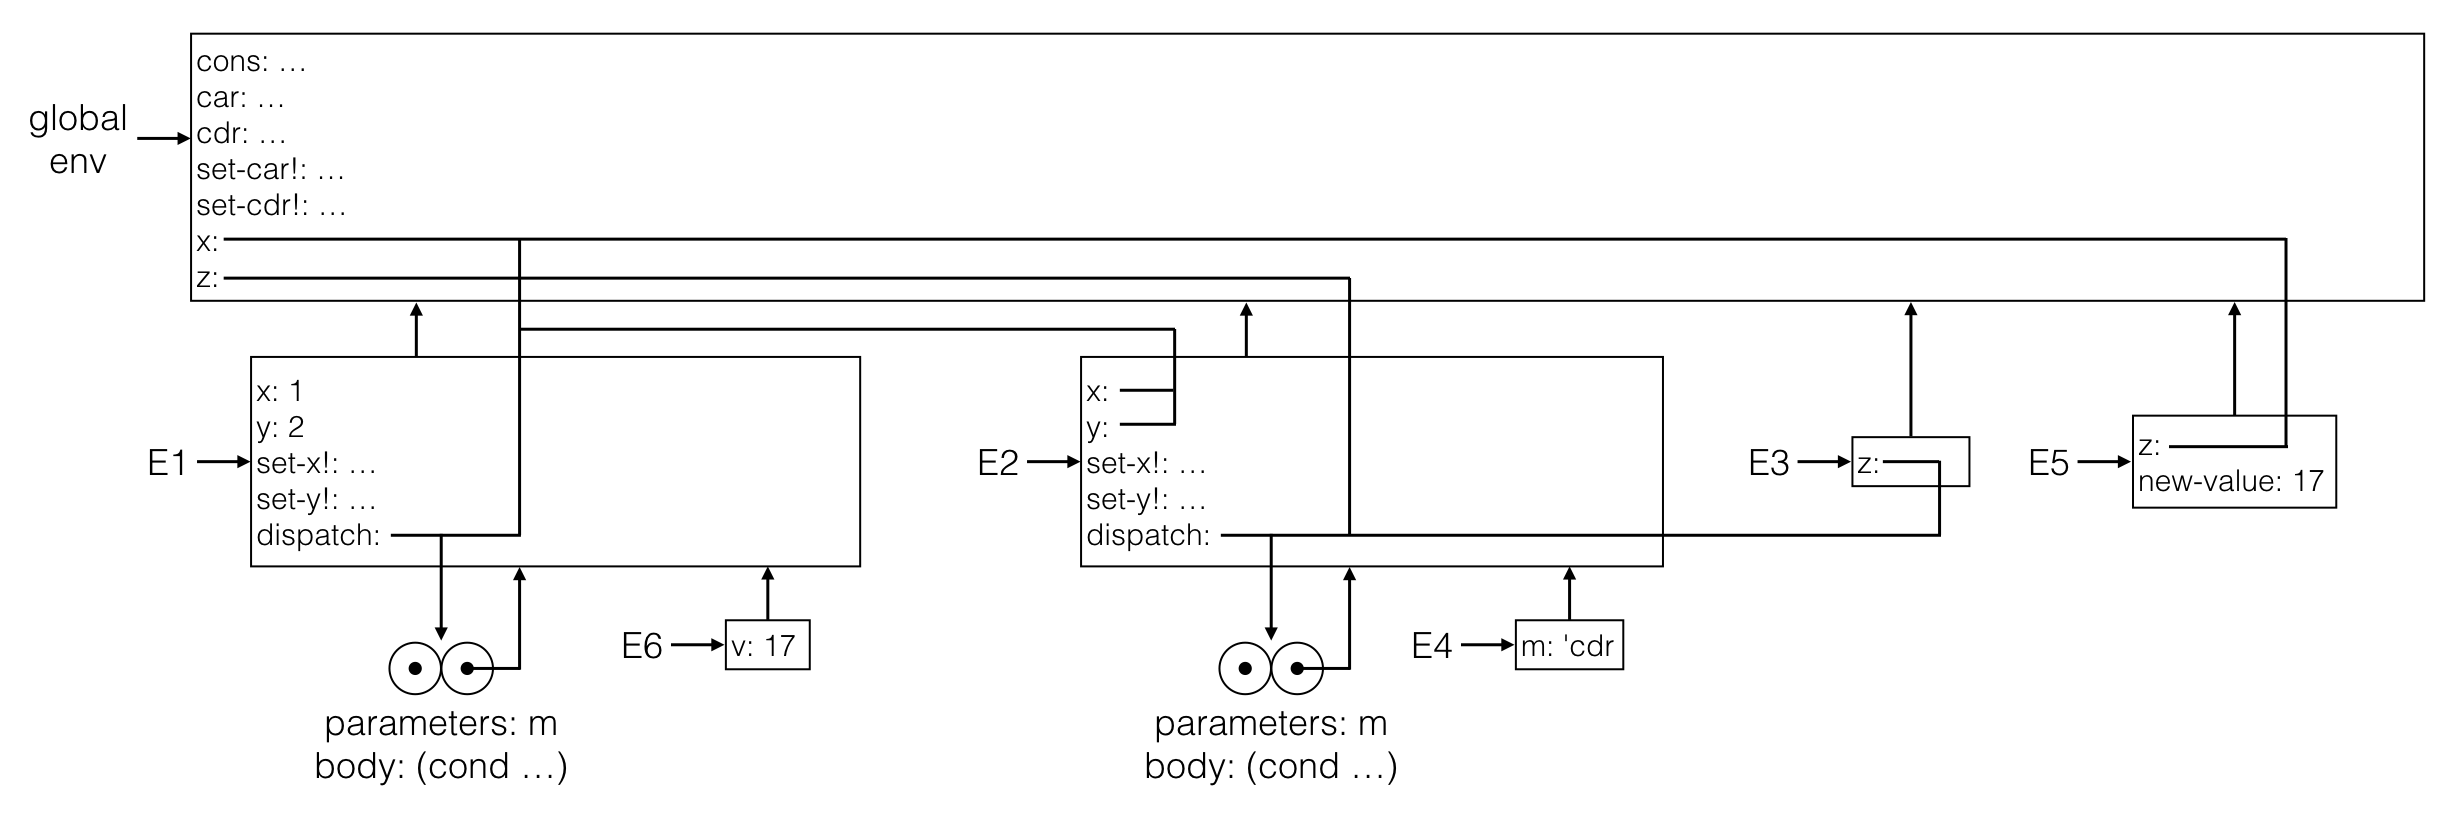
\includegraphics[width=15cm]{ex-3.20-2.png}
    \caption{Effect of \textbf{(set-car! (cdr z) 17)}.}
\end{figure}

\begin{figure}[h!]
    \centering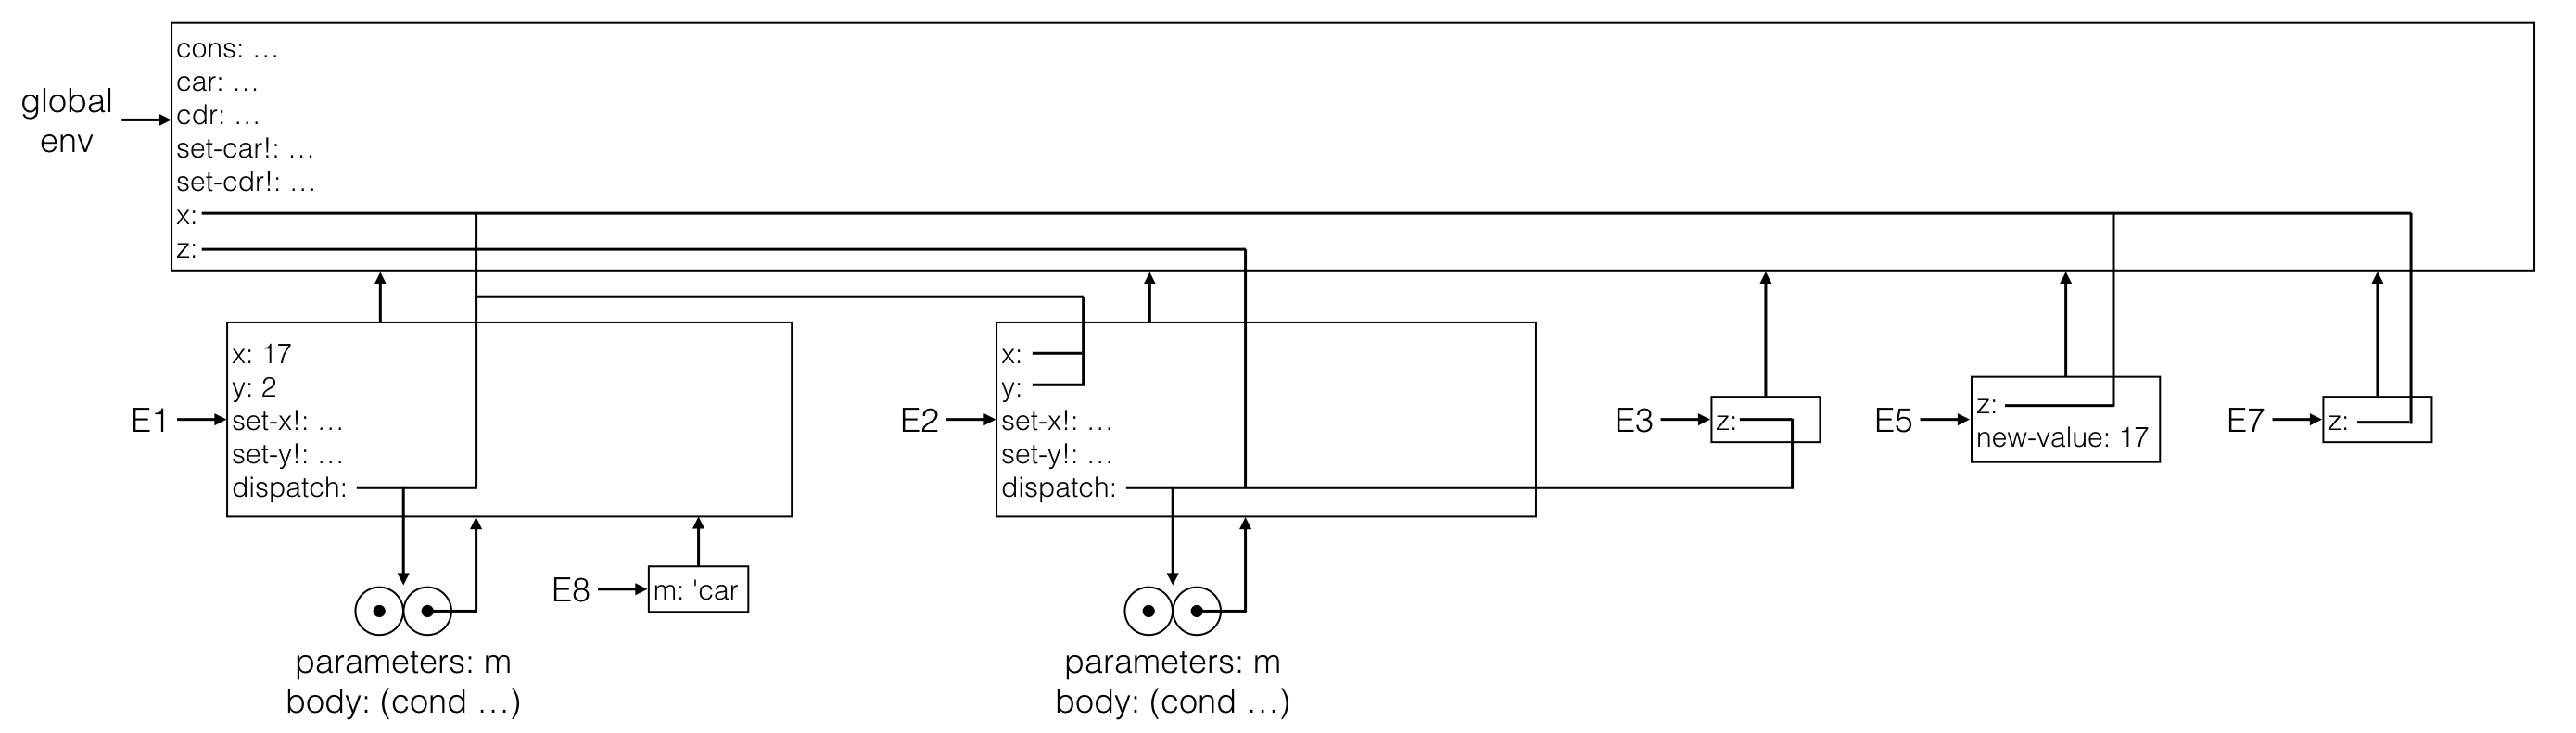
\includegraphics[width=15cm]{ex-3.20-3.png}
    \caption{Effect of \textbf{(car x)}.}
\end{figure}

\end{document}
